\subsection{Wire with periodical curvature distribution}

Here, we consider a flat anisotropic FM nanowire with a fixed cross-section of area $S$ and periodically repeated semicircles of curvature $\varkappa_0$~\cite{Korniienko19b}, i.e. meander geometry [see Fig.~\ref{fig:Geometries_n_curvatures}(c)]. The spatial distribution of the curvature of such a wire is the square-wave function $\varkappa(\xi) = (-1)^{\lfloor\xi/\xi_0\rfloor}\varkappa_0$ with period $2\xi_0$ and $\xi_0=\pi/\varkappa_0$ being the length of a semicircle. Here $\lfloor x \rfloor$ defines the integer part of $x$.

\subsubsection{Equilibrium state}

 Similarly to the case of the box-function curvature profile discussed in Sec.~\ref{sec:box_curvature_equilibrium}, here we also have a planar magnetization distribution within wires plane~\cite{Korniienko19b}. The ground state is described by Eqs.~\eqref{eq:Theta-Phi-statics} with azimuthal angle $\phi$ defined as
\begin{equation}\label{eq:phi_meander}
\phi_0 = (-1)^\lambda \text{am}\left[\frac{\xi-\xi_0\left(\lambda+1/2\right)}{k},ik\right],\quad \lambda=\lfloor \xi/\xi_0 \rfloor,\quad k=\frac{1}{\sqrt{\varkappa_0^2-\sin^2\varphi_0}},
\end{equation}
where $\varphi_0=|\phi\left(n\xi_0\right)|$ is maximal value of the function $\phi(\xi)$ [see Fig.~\ref{fig:meander}(b)], it is determined by the equation $2kF(\varphi_0,ik) = \xi_0$, where $F(x,y)$ is elliptic integral of the first kind~\cite{NIST10} and the modulus $k = k(\varphi_0)$ is defined in~\eqref{eq:phi_meander}. One should note that the curvature amplitude $\varkappa_0$ is the only parameter which controls the system. The maximal deviation $\varphi_0$ from the tangential direction takes place in points of junction of two semicircles, this is because of the curvature jump. Depending on the $\varkappa_0$ one obtains two different behaviors~\cite{Korniienko19b}: (i) In the limit case of small curvature $\varkappa_0\ll1$ and due to the easy-tangential anisotropy the wire is magnetized practically tangentially except the junction points, where the magnetization demonstrates the small deviations of amplitude $\varphi_0\approx\varkappa_0$. (ii) In the opposite case of large curvature $\varkappa_0\gg1$ exchange interaction is dominating and results in quasi uniform magnetization aligned with $x$-axis with $\varphi_0\lesssim\pi/2$.

%==================================================================\
\begin{figure}[t]
	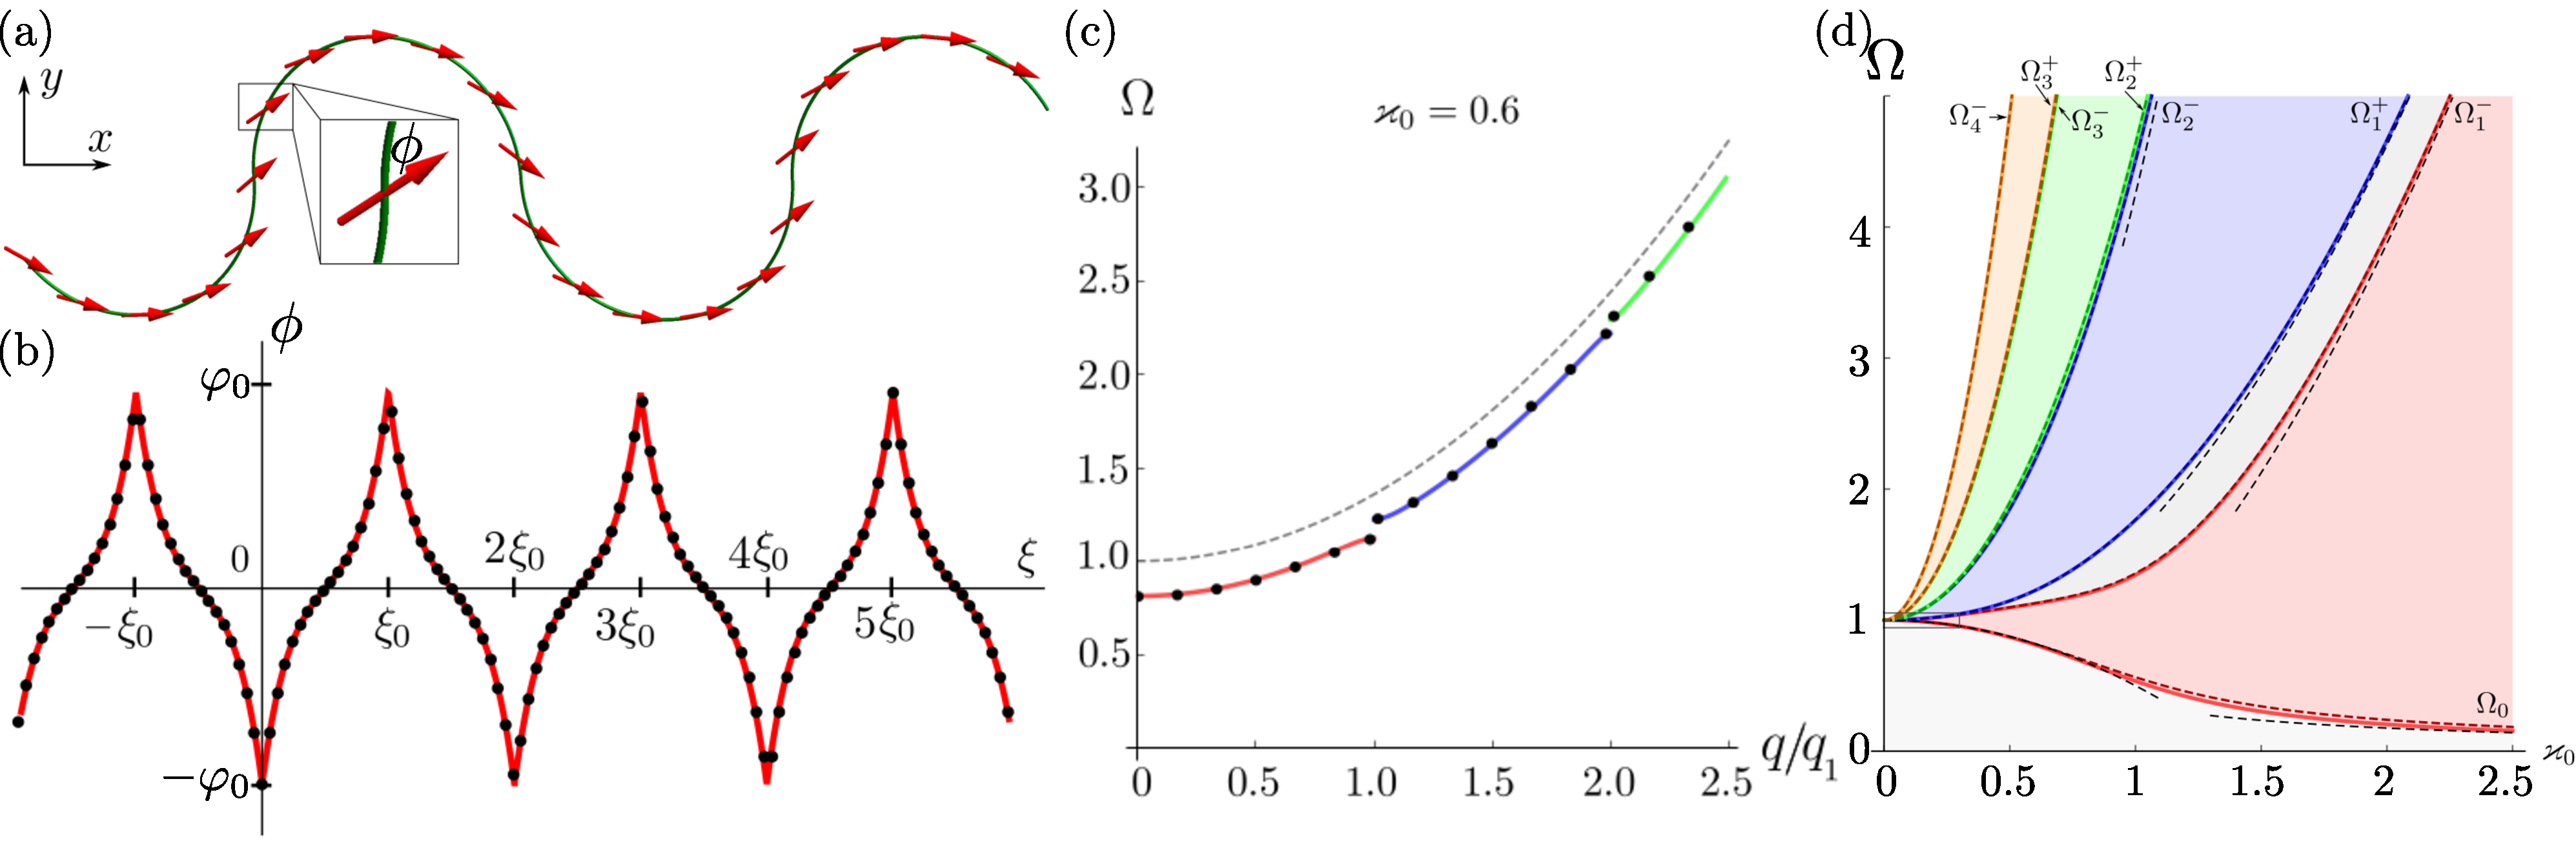
\includegraphics[width=\textwidth]{fig_meander}
	\caption{\label{fig:meander}%
		\textbf{Meander shaped wire:} (a) Spatial distribution of magnetization (red arrows) along the wires with the shape of meander; the inclination angle $\phi$ is shown in insets. (b) Azimuthal angle $\phi$ as function of arc length for meander shaped wire with $\varkappa_0=0.6$: line -- analytical solution, dots -- results of numerical simulations. (c) Dispersion relation for meander nanowire with  $\varkappa_0=0.6$. The dashed line shows the dispersion relation of a straight wire ($\varkappa_0=0$). The wavevector is normalized by $q_1=\varkappa_0$ corresponding to the edge of the first Brillouin zone. (d) The band structure as function of $\varkappa_0$. The first four bands of the magnon conductance are shown by different colours and gaps are shown by grey shading. Solid and dashed thick lines correspond to the exact numerical solution and to the approximations~\eqref{eq:band_gaps_meander}, respectively. Adapted with permission from~\cite{Korniienko19b}.}
\end{figure}
%==================================================================/

\subsubsection{Band structure}

The linear dynamics of magnetization in the meander shaped nanowire can be described by the generalized Schr\"odinger equation~\eqref{eq:Schroedinger} with geometry-induced potentials
\begin{equation} \label{eq:V-n-W_meander}
W(\xi) = \frac{\varkappa_0}{k}\sqrt{1+k^2\sin^2\phi_0}-\frac{1}{2}\left(\frac{1}{k^2}+\varkappa^2_0\right),\quad U(\xi) = W-2\sin^2\phi_0,
\end{equation}
where $\phi_0$ is determined in~\eqref{eq:phi_meander}. One should note that potentials $V(\xi)=V(\xi+\xi_0)$ and $W(\xi)=W(\xi+\xi_0)$ have twice as small period as $\phi_0(\xi)$ has, this is because the dependence on $\xi$ is reduced to the dependence on $\sin^2\phi_0(\xi)$ in~\eqref{eq:V-n-W_meander}. The periodic potential in a quantum mechanical Schr\"odinger equation always produces the band structure. Therefore, one can consider the the meander shaped wire as an magnonic crystal. In contrast to the straight wire, the dispersion relation for a given curvature $\varkappa_0>0$ demonstrates the frequency reduction and appearance of the band structure, see Fig.~\ref{fig:meander}(c). The band gap edges can be estimated as~\cite{Korniienko19b}
\begin{equation}
\Omega^{\pm}_\nu\approx\sqrt{\left(q^2_\nu+1+\mathcal{U}_0\mp \mathcal{U}_\nu\right)^2-\left(\mathcal{W}_0\mp \mathcal{W}_\nu\right)^2}, \quad \nu\in\mathbb{N}.
\end{equation}
Here $\Omega^{+}_\nu$ and $\Omega^{-}_\nu$ correspond to the top and bottom edges of the $\nu$-th gap, respectively, $q_\nu = \nu\varkappa_0$ is a wavevector which corresponds to the edge of the $\nu$-th Brillouin zone, coefficients $\mathcal{U}_n$ and $\mathcal{W}_n$ denote Fourier components of the effective potentials $U$ and $W$, respectively. The size of the main gap $\Omega_0$ can be approximated as~\cite{Korniienko19b}
\begin{equation}\label{eq:band_gaps_meander}
\Omega_0\approx\sqrt{\left(1+\mathcal{U}_0\right)^2-\mathcal{W}_0^2}
\end{equation}
with Fourier coefficients
\begin{equation}
	\mathcal{U}_0 \approx -\frac{\varkappa_0^2}{2}\tanh^2\frac{\xi_0}{2}, \quad \mathcal{W}_0 \approx -\frac{\varkappa_0^2}{2}\left[1+\frac{1}{\cosh^2\frac{\xi_0}{2}} - \frac{4}{\xi^2}\tanh\frac{\xi_0}{2}\right].
\end{equation}
For the case of the small curvature amplitude $\varkappa_0\ll 1$ one obtains $\Omega_0\approx1 - \varkappa_0^2/2$, while for the large curvature amplitude $\varkappa_0\gg1$ we have $\Omega_0\approx 1/\left(2\sqrt{2}\varkappa_0\right)$, see Fig.~\ref{fig:meander}(d).